\scanpage{63}
% L01
\[\Gamma^{\unsure{0|\circ}}_{\infty,3}\simeq\mathrm{SL}(2,\mathbb{Z})/\pm1\]
% L02-03
\diagram{\begin{tikzcd}[ampersand replacement=\&]
\Gamma^0_{n,3}\arrow[r,"\text{épi}"]\&\mathrm{SL}(2,\mathbb{Z}_n)/\pm1\arrow[d,equal]\\
\&\deleted{\unsure{\mathrm{GL}(2,\mathbb{Z}_n)|\mathrm{PSL}(2,\mathbb{Z}_n)}}
\end{tikzcd}}
$(n\ge\unsure{2|3})$ (iso \uline{ssi $n\le5$})
% Rounded marginal callout, with its tail towards the condition n<=5.
\margin{\figure{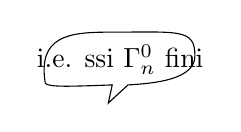
\begin{tikzpicture}[x=1cm,y=1cm]
\draw (0,.2)..controls (-.1,.8) and (.3,.85)..(.8,.85)
 ..controls (1.7,.85) and (1.9,.9)..(1.9,.55)
 ..controls (1.9,.25) and (1.4,.2)..(1.05,.18)
 --(.8,-.05)--(.85,.18)
 ..controls (.3,.16) and (.05,.15)..(0,.2);
\node[align=center] at (.95,.5) {i.e. ssi $\Gamma_n^0$ fini};
\end{tikzpicture}}}
% L04-05
l'étudier pour $n=$\uline{$2,3,4,5,6$}

% Above table, cancelled heading
\deleted{ordre $\Gamma_{n,3}$}
% L06-11, table
\diagram{$\begin{array}{c|l|c|l}
n&\text{ordre }\Gamma^0_{n,3}&\text{ordre }\mathrm{SL}(2,\unsure{\mathbb{Z}/n|\mathbb{Z}_n|\mathbb{Z}/n\mathbb{Z}})/\pm1&\\\hline
2&(\unsure{\mathfrak{S}_3|G_3})\ 6&6&\text{cas 3-dièdre?}\\\hline
3&(\unsure{\mathfrak{A}_4|\mathcal{A}_4})\ 12&12&\text{tétraèdre }\unsure{\text{or.}|\text{or}}\\\hline
4&(\mathfrak{S}_4)\ 24&24&\text{\uline{cube orienté}}\\\hline
5&(\mathfrak{A}_5)\ 60&60&\text{icos. orienté}\\\hline\hline
6&(\mathbb{Z}_6\cdot\mathbb{Z}^2)\ \infty&72&\begin{gathered}\text{pav. en }\unsure{\text{triangles}}\\\text{\uline{\unsure{équilat.} orienté}}\\\text{\uline{du plan}}\end{gathered}
\end{array}$}

% Right of table, upper formula
\[
\begin{aligned}
\operatorname{Card}\mathrm{SL}(2,\mathbb{F}_q)&=(q+1)q(q-1)\\
&=q(q^2-1)
\end{aligned}
\]
% Right of table, lower formula
\[
\begin{aligned}
\operatorname{Card}\mathrm{SL}(2,\mathbb{Z}/p^{\unsure{n|\nu}}\mathbb{Z})&=\\
(\operatorname{card}\mathrm{SL}(2,\mathbb{F}_p))\,p^{3(n-1)}&
\end{aligned}
\]
% archive sheet number: 62
